\part{El Software}

\paragraph{Software}
% Instrucciones de ordenador que cuando se ejecutan proporcionan la función y el comportamiento deseado, estructuras de datos que facilitan a los programas manipular adecuadamente la información, y documentos que describen la operación y el uso de los programas.
% \\\\
\textit{Pressman} define el software como el conjunto de \textbf{código, estructuras de datos y documentación} asociados a un sistema computacional. Es habitualmente, el componente de un sistema que presenta mayores problemas durante el desarrollo.

\paragraph{Ingeniería del Software}
Es aquella disciplina que se encarga de \uline{establecer un orden en el desarrollo de sistemas de software}.

\paragraph{Crisis del software}
Durante los primeros años del desarrollo del software, al no utilizarse metodología ninguna, los programas contenían numerosos errores e inconsistencias que obligaban a realizar continuas modificaciones. Al final, se hacía más rápido y, por lo tanto barato, empezar de cero a realizar un software, en lugar de modificar uno ya existente, pero que acabaría presentando los mismos problemas.

\section{Características}
El software se diferencia principalmente por presentar una \textbf{naturaleza lógica} (es inmaterial); por ello, se dice que el \textbf{software se desarrolla, no se fabrica} en sentido estricto. A pesar de presentar muchas similitudes con los productos de otras ingenierías (\textit{fases de análisis, diseño, etc.}), el software se diferencia por lo siguiente:
\begin{enumerate}

    \item \textbf{Costes de replicación negligibles}:
          En el caso del software, la mayor parte de la inversión se concentra en las fases de ingeniería previas a la producción, dado que, al ser un producto inmaterial, la replicación del producto no presenta problemas técnicos, no requiere un control individualizado, y el coste unitario resulta prácticamente nulo.
          \begin{figure}[h]
            \centering
            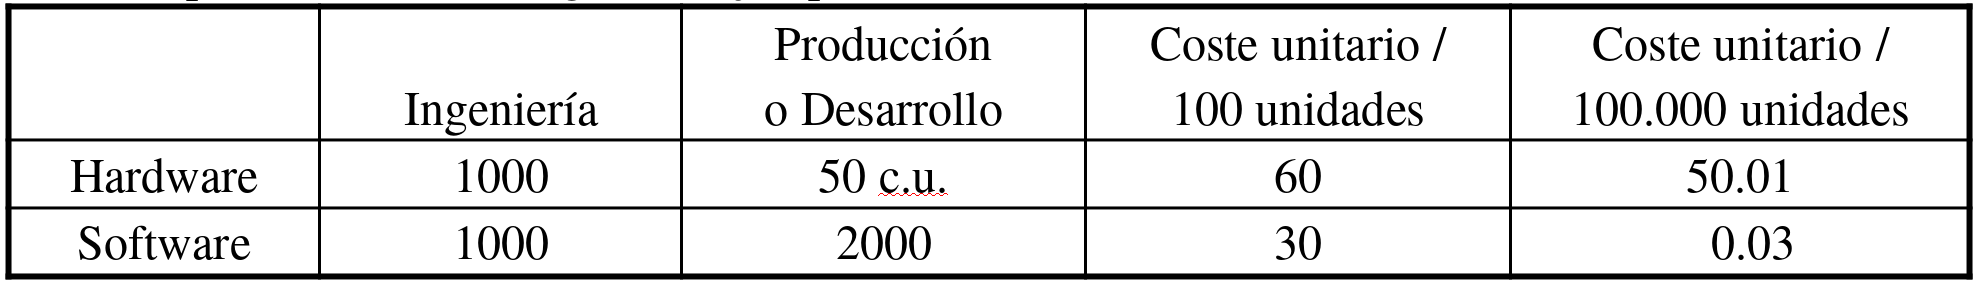
\includegraphics[width=0.8\textwidth]{Resources/Tema1/CostesProduccion.png}
            \caption{Influencia de los costes de ingeniería en el coste total del producto.}
        \end{figure}
          
    \item \textbf{Curva de fallos con respecto al tiempo diferente}:
          El software no se estropea con el tiempo; sin embargo es común aplicar ciertos cambios al mismo durante su ciclo de vida debidos al mantenimiento. Por ello, es probable que se introduzcan nuevos errores, que se acumulan con el tiempo por introducir más problemas antes de solucionar los ya existentes, degradando así la calidad. \textbf{El software no se estropea, pero se deteriora}.
          \begin{figure}[h]
            \centering
            \includegraphics[width=0.4\textwidth]{Resources/fallosSoftwareReales.png}
            \includegraphics[width=0.4\textwidth]{Resources/fallosHardware.png}
            \caption{Curva de fallos del Software (izquierda) y del Hardware (derecha). Obsérvese como, en el caso del software, el índice de fallos se va acumulando; idealmente, el software solo presentaría fallos al principio de su vida, por errores no detectados durante el desarrollo.}
        \end{figure}
    \item \textbf{Baja reutilización de las partes}:
          Por lo general el software se construye a medida como un conjunto, provocando que la reutilización sea baja; consecuentemente, se perjudica el desarrollo del software. Existe una tendencia al alza en la reutilización de artefactos (no tienen por qué ser código) gracias a:
          \begin{itemize}
              \item La elaboración de librerías y \textit{frameworks}.
              \item Aplicación de técnicas de programación estructurada, modular y orientada a objetos.
              \item Aplicación de patrones de diseño, que supone el poder reutilizar diseños, el lugar de solo código.
          \end{itemize}
          Una empresa debería identificar los artefactos reutilizables con los que cuente, para que sus empleados los utilicen.
\end{enumerate}

\section{Atributos deseables en el software}
Todo software debería contar con las siguientes características:
\begin{itemize}
    \item \textbf{Mantenibilidad}: Facilidad para realizar cambios.
    \item \textbf{Confiabilidad}: Capacidad para seguir funcionando de manera segura y correcta.
    \item \textbf{Eficiencia}: Utilización de la mínima cantidad necesaria de recursos.
    \item \textbf{Usabilidad}: Facilidad con la que las personas utilizan el software.
\end{itemize}

\subsection{Aplicaciones del software}
Es difícil clasificarlas y, realmente, carece de mucho valor hacerlo. \textit{Pressman} lo hace de la siguiente forma:
\begin{itemize}
    \item \textbf{Software de sistemas}: Sirven a otros programas.
    \item \textbf{Software de aplicación}: Programas independientes que resuelven una necesidad específica; es decir, están hechos a medida.
    \item \textbf{Software científico y de ingeniería}: ``Devoradores de números''.
    \item \textbf{Software empotrado}: Reside en una memoria de sólo lectura de pequeños chips, y con funciones limitadas y muy específicas.
    \item \textbf{Software de línea de productos}: \textit{Middleware}; cuentan con una capacidad específica que muchos clientes pueden usar (\textit{por ejemplo: procesador de textos}).
    \item \textbf{Aplicaciones web}.
    \item \textbf{Inteligencia artificial}: \textit{Redes neuronales} (\textbf{NO} son máquinas de estados).
\end{itemize}
El objetivo de todo software es desempeñar una determinada función \uline{cumpliendo una serie de requisitos}.

\section{Software heredado}
Se trata de software \textbf{desarrollado hace décadas} que además \textbf{ha ido sufriendo cambios} a lo largo del tiempo para adaptarse a los requisitos cambiantes del negocio. Estos dos factores hacen que sea habitual que \textbf{le falte calidad}, no necesariamente por un desarrollo descuidado, sino porque \textbf{su proceso de desarrollo se ha quedado desfasado}. Por ejemplo, en su momento pudieron tomarse decisiones consideradas como malas prácticas hoy en día, como restar importancia a tener la documentación al día.

Por lo tanto, sus diseños son con frecuencia imposibles de extender, junto con un código complicado, documentación escasa o incluso inexistente, falta de historial de cambios, y pruebas sin archivar. Así, es \uline{muy difícil, y por lo tanto caro, de tratar, siendo además normalmente crítico para los negocios} (\textit{por ejemplo: COBOL}).


\textit{Pressman} aconseja tocarlo lo mínimo posible, al menos mientras no sea necesario.

\section{Principales problemas asociados a la producción del software}
Muchos expertos argumentan que la crisis del software nunca se ha solucionado, y es que esta ingeniería arrastra desde hace tiempo los siguientes \textbf{problemas crónicos}, causados por las propias características del software y por los errores de quienes intervienen en su producción:
\begin{enumerate}
    \item \textbf{Imprecisión en la planificación, y en la estimación de costes temporales y monetarios}: Es \uline{frecuente que surjan imprevistos al abordar proyectos de cierta complejidad}, dando lugar a desviaciones. Además, \uline{sin una planificación detallada, es imposible hacer una estimación de costes e identificar las tareas conflictivas}. Entre las causas podemos citar la falta de recogida de datos de proyectos anteriores (no acumular experiencia), y la tradicional falta de experiencia de los gestores de proyecto (gente que no tiene ni idea de software gestionando proyectos, o incluso viceversa fuera del contexto de la Ingeniería del Software).
    \item \textbf{Baja productividad}: Los proyectos de software tienen a una \uline{duración mayor a lo esperada} y, por lo tanto, \uline{mayores costes}, y menor productividad y beneficios. Entre los múltiples motivos, se encuentran las especificaciones ambiguas o incorrectas, la poca comunicación con el cliente hasta la entrega, con sus consecuentes cambios de última hora, y la falta de documentación. Este problema culmina con que sea más costoso realizar una modificación sobre un programa que el rehacerlo.
    \item \textbf{Mala calidad}: El que las especificaciones sean ambiguas o incorrectas, junto con falta de realización de pruebas exahustivas, propicia la \uline{entrega de software con muchos errores}, y por lo tanto incrementa los costes durante el mantenimiento.
    \item \textbf{Insatisfacción del cliente}: Debido a los problemas anteriores, los clientes suelen quedar poco satisfechos con los resultados.
\end{enumerate}